\section{Thử nghiệm mô hình}

\subsection{Ảnh hưởng của Patch Size}

\begin{table}[H]
\centering
\caption{So sánh các kích thước patch}
\label{tab:patch_size}
\begin{tabular}{|c|c|c|c|c|}
\hline
\textbf{Patch Size} & \textbf{Accuracy} & \textbf{ROC-AUC} & \textbf{Thời gian huấn luyện} & \textbf{Số tham số} \\
\hline
1×1 (pixel-wise) & 98.23\% & 99.78\% & 12.5s & 25,348 \\
\hline
\textbf{3×3 (baseline)} & \textbf{98.86\%} & \textbf{99.98\%} & 15.2s & 36,676 \\
\hline
5×5 & 98.67\% & 99.89\% & 28.3s & 52,484 \\
\hline
7×7 & 98.29\% & 99.86\% & 41.2s & 71,108 \\
\hline
\end{tabular}
\end{table}

\begin{figure}[H]
    \centering
    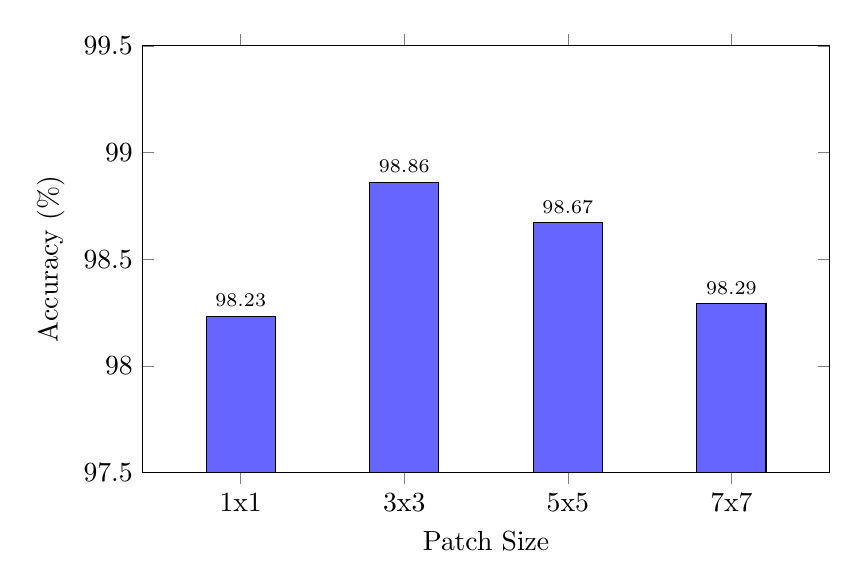
\begin{tikzpicture}
        \begin{axis}[
            ybar,
            width=0.85\textwidth,
            height=7cm,
            ylabel={Accuracy (\%)},
            xlabel={Patch Size},
            symbolic x coords={1x1, 3x3, 5x5, 7x7},
            xtick=data,
            ymin=97.5,
            ymax=99.5,
            bar width=25pt,
            nodes near coords,
            nodes near coords align={vertical},
            every node near coord/.append style={font=\scriptsize},
            enlarge x limits=0.2,
        ]
        \addplot[fill=blue!60] coordinates {
            (1x1, 98.23)
            (3x3, 98.86)
            (5x5, 98.67)
            (7x7, 98.29)
        };
        \end{axis}
    \end{tikzpicture}
    \caption{So sánh Accuracy theo các Patch Size}
    \label{fig:patch_size_comparison}
\end{figure}

Qua Bảng~\ref{tab:patch_size} và Hình~\ref{fig:patch_size_comparison}, có thể rút ra một số nhận xét quan trọng. Với patch size 1×1 (pixel-wise), mô hình đạt accuracy 98.23\%, cho thấy chỉ riêng thông tin phổ tại mỗi pixel đã đủ để phân biệt các lớp biến động rừng với độ chính xác cao, tuy nhiên cách tiếp cận này bỏ qua thông tin ngữ cảnh không gian. Patch size 3×3 đạt kết quả tốt nhất (98.86\% accuracy, 99.98\% ROC-AUC) với mức tăng thời gian huấn luyện chấp nhận được (+2.7 giây so với 1×1), cho thấy kích thước này cân bằng tốt giữa việc khai thác ngữ cảnh không gian địa phương và tránh nhiễu từ các pixel xa.

Đối với patch size 5×5 và 7×7, accuracy giảm dần (98.67\% và 98.29\%) mặc dù số tham số mô hình tăng đáng kể, cho thấy với độ phân giải 10m của Sentinel-2, ngữ cảnh không gian quá rộng (50-70m) có thể đưa vào nhiễu từ các lớp phủ lân cận, đặc biệt tại các vùng ranh giới. Thời gian huấn luyện tăng gần tuyến tính với số tham số, từ 12.5s (1×1) lên 41.2s (7×7), cho thấy chi phí tính toán tăng đáng kể khi mở rộng patch size mà không đem lại cải thiện về accuracy. Do đó, có thể kết luận rằng patch size 3×3 là tối ưu cho bộ dữ liệu này, đạt được sự cân bằng tốt nhất giữa độ chính xác, thời gian huấn luyện và khả năng khai thác ngữ cảnh không gian.

\subsection{Ảnh hưởng của nguồn dữ liệu}

\begin{table}[H]
\centering
\caption{Nghiên cứu loại trừ các nguồn dữ liệu}
\label{tab:data_sources}
\begin{tabular}{|l|c|c|c|}
\hline
\textbf{Cấu hình} & \textbf{Số đặc trưng} & \textbf{Accuracy} & \textbf{ROC-AUC} \\
\hline
Chỉ Sentinel-2 (delta) & 7 & 87.65\% & 94.12\% \\
\hline
Sentinel-2 (trước + sau + delta) & 21 & 93.42\% & 97.58\% \\
\hline
Chỉ Sentinel-1 (trước + sau + delta) & 6 & 83.27\% & 91.45\% \\
\hline
\textbf{S1 + S2 (tất cả)} & \textbf{27} & \textbf{98.86\%} & \textbf{99.98\%} \\
\hline
\end{tabular}
\end{table}

\begin{figure}[H]
    \centering
    \begin{tikzpicture}
        \begin{axis}[
            ybar,
            width=0.95\textwidth,
            height=7cm,
            ylabel={Accuracy (\%)},
            symbolic x coords={S2 (delta), S2 (tất cả), S1 (tất cả), S1+S2 (tất cả)},
            xtick=data,
            xticklabel style={rotate=15, anchor=east, font=\small},
            ymin=80,
            ymax=100,
            bar width=22pt,
            nodes near coords,
            nodes near coords align={vertical},
            every node near coord/.append style={font=\scriptsize},
            enlarge x limits=0.15,
        ]
        \addplot[fill=orange!70] coordinates {
            (S2 (delta), 87.65)
            (S2 (tất cả), 93.42)
            (S1 (tất cả), 83.27)
            (S1+S2 (tất cả), 98.86)
        };
        \end{axis}
    \end{tikzpicture}
    \caption{So sánh Accuracy theo các nguồn dữ liệu}
    \label{fig:data_sources_comparison}
\end{figure}

Qua Bảng~\ref{tab:data_sources} và Hình~\ref{fig:data_sources_comparison}, có thể rút ra các nhận xét quan trọng về vai trò của từng nguồn dữ liệu. Sentinel-2 đóng vai trò chủ đạo trong phân loại biến động rừng, thể hiện qua việc chỉ với dữ liệu Sentinel-2 delta (7 kênh biến động), mô hình đã đạt 87.65\% accuracy, và khi bổ sung đầy đủ dữ liệu trước, sau và delta (21 kênh), accuracy tăng lên 93.42\%, khẳng định tầm quan trọng của thông tin quang phổ và phương pháp phân tích 2 thời điểm trong phát hiện biến động. Trong khi đó, Sentinel-1 đơn lẻ có hiệu suất thấp nhất (83.27\% accuracy với 6 kênh); dữ liệu ra-đa khẩu độ tổng hợp tuy có ưu điểm không bị ảnh hưởng bởi mây và có khả năng quan sát cấu trúc rừng, nhưng độ phân giải phổ hạn chế (chỉ có VV và VH) khiến việc phân biệt các lớp phủ trở nên khó khăn hơn đáng kể so với dữ liệu quang học đa phổ.

Sự kết hợp S1+S2 cho kết quả tốt nhất (98.86\% accuracy, 99.98\% ROC-AUC), vượt trội đáng kể so với việc chỉ sử dụng Sentinel-2 (+5.44\%), cho thấy dữ liệu ra-đa bổ sung thông tin cấu trúc và độ ẩm mà dữ liệu quang học không nắm bắt được, đặc biệt hữu ích cho việc phân biệt rừng có mật độ tán khác nhau, phát hiện vùng rừng suy thoái chưa thể hiện rõ trên ảnh quang học, và cải thiện phân loại trong điều kiện có mây một phần. Bên cạnh đó, đóng góp của thông tin thời gian là đáng kể khi accuracy tăng từ 87.65\% (chỉ delta) lên 93.42\% (đầy đủ trước + sau + delta), khẳng định giá trị của việc khai thác thông tin đa thời gian trong phát hiện biến động.

Từ các kết quả trên, có thể kết luận rằng việc kết hợp Sentinel-1 và Sentinel-2 cho kết quả tối ưu nhất. Dữ liệu ra-đa và quang học có tính bổ sung cao: Sentinel-2 cung cấp thông tin chi tiết về thành phần hóa học và sinh lý của thực vật thông qua các kênh quang phổ, trong khi Sentinel-1 cung cấp thông tin về cấu trúc và độ ẩm của tán rừng. Sự kết hợp này đặc biệt phù hợp cho giám sát rừng ngập mặn ven biển, nơi điều kiện thời tiết thường xuyên có mây và sương mù.
